\documentclass[10pt]{beamer}
\setbeamerfont{structure}{family=\rmfamily} 
\usepackage{hyperref}
\usepackage{CJKutf8}
\usepackage{amsmath}
\usepackage{amssymb}
\usepackage{amsthm}
\usepackage{graphicx}
\usepackage{graphics}
\usepackage{hyperref}
\renewcommand{\baselinestretch}{1.5}
\beamertemplatenavigationsymbolsempty
\setbeamertemplate{blocks}[rounded][shadow=true]
\setbeamertemplate{bibliography item}[text]
\setbeamertemplate{caption}[numbered]
\usetheme{default}
\usecolortheme{seahorse}
\mode<presentation>
{
   \setbeamercovered{transparent}
   \setbeamertemplate{items}[circle]
   \setbeamertemplate{theorems}[numbered]
   \setbeamertemplate{footline}[frame number]

}

\usepackage{tikz}
\usetikzlibrary{arrows}
\usetikzlibrary{trees}

\tikzstyle{every node}=[draw=black,thick,anchor=west]
\tikzstyle{selected}=[draw=red,fill=red!30]
\tikzstyle{optional}=[dashed,fill=gray!50]

\tikzset{
  treenode/.style = {align=center, inner sep=0pt, text centered, font=\sffamily},
  arn_n/.style = {treenode, rectangle, white, draw=black, fill=black, minimum width=2em, minimum height=2em},
  arn_r/.style = {treenode, rectangle, red, draw=red,very thick, minimum width=2em, minimum height=2em},
  arn_x/.style = {treenode, rectangle, draw=black, minimum width=0.5em, minimum height=0.5em}
}

\begin{document}
\begin{CJK*}{UTF8}{gbsn}
\title {\bfseries{\sc Introduction of \LaTeX}}
\author[Nano]{Nano}
\institute{artiano@hotmail.com}
\date{\small 2017-07-20} 
%--------------------------------------------------------------------------%
\begin{frame}
\titlepage
\end{frame}
%---------------------------------------------------------------------------%
\section*{Outline}
\begin{frame}
\frametitle{\sc{outline}}  
\tableofcontents
\end{frame}
%---------------------------------------------------------------------------

\section{\LaTeX}
    \subsection{\sc{what is {\LaTeX}}}
    \subsection{\sc{syntactic structure of \LaTeX}}
\begin{frame}
\frametitle{\LaTeX}
    \begin{itemize}
    \item {What is {\LaTeX}}
        \begin{itemize}
            \item LaTeX is a document preparation system for high-quality typesetting. It is most often used for medium-to-large technical or scientific documents but it can be used for almost any form of publishing.
            \item TeX (/ˈtɛx/ tekh as in Greek, but often pronounced /ˈtɛk/ tek in English) is a typesetting system designed and mostly written by Donald Knuth and released in 1978.(From Wikipedia)
        \end{itemize}
    \item {Syntactic structure of \LaTeX}
        \begin{itemize}
            \item Macro and Environment
            \item \href{https://www.sharelatex.com/learn/Mathematical_expressions}{Math environment}
            \item \href{https://www.sharelatex.com/learn/Chinese}{Chinese support}
        \end{itemize}
    \end{itemize}
\end{frame}
%---------------------------------------------------------------------------%
\section{\sc{implementation of {\LaTeX } math environment}}
    \subsection{\sc{resources}}
    \subsection{\sc{parsing algorithm}}
\begin{frame}
\frametitle{\sc{resources}}
\begin{itemize}
    \item \href{http://www.unicode-table.com/}{Charset}
    \item Typeface information (Metrics, \href{http://en.wikipedia.org/wiki/Kerning}{Kerning}, \href{http://en.wikipedia.org/wiki/Typographic_ligature}{Ligature}) \\
        \includegraphics[scale=.16]{glyph_metrics.png}
    \item \href{http://www.tug.org/texlive//devsrc/Master/texmf-dist/doc/latex/base/encguide.pdf}{{\LaTeX } font encodings}
\end{itemize}
\end{frame}
\begin{frame}{\sc{parsing algorithm}}
In {\LaTeX } \text{[$ x=\backslash frac\{-b\backslash pm \backslash sqrt \{ b \wedge 2-4ac \} \} \{ 2a \} $]} As an example:
$$x=\frac{-b\pm\sqrt{b^2-4ac}}{2a}$$
\begin{itemize}
    \item Atomization\\
    We got a sequence of all atomic elements, {$x, =, -, \ldots$}
    \item Generate syntax tree\\
    We got all information we need to place the atomic elements
    \item Visualize\\
    Inflate the generated tree and draw
\end{itemize}
\end{frame}

\begin{frame}{\sc{syntax tree}}
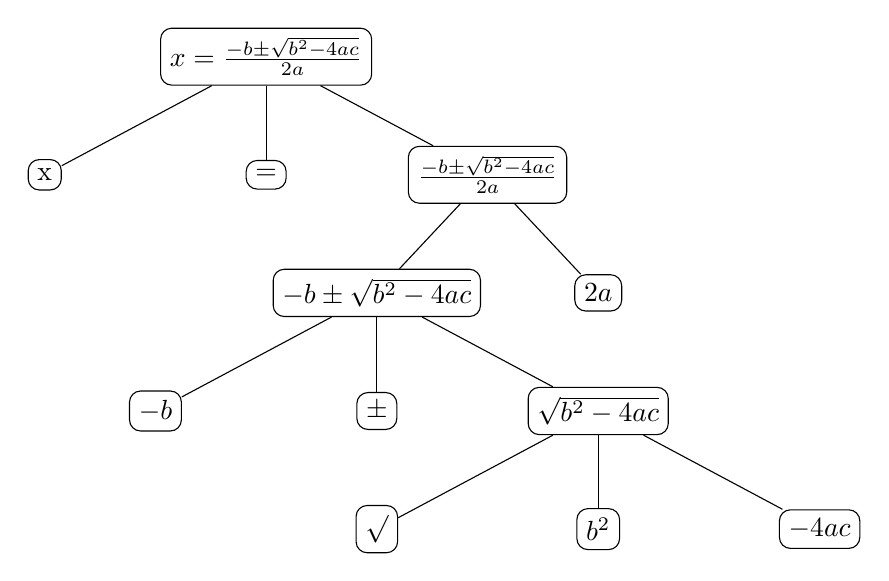
\begin{tikzpicture}[sibling distance=8em,
  every node/.style = {shape=rectangle, rounded corners,
    draw, align=center}]]
\node{$x = \frac{-b\pm\sqrt{b^2-4ac}}{2a}$}
    child{ node {x} }
    child{ node {=} }
    child{ node {$\frac{-b\pm\sqrt{b^2-4ac}}{2a}$}
        child{ node {$-b\pm\sqrt{b^2-4ac}$}
            child{ node {$-b$} }
            child{ node {$\pm$} }
            child{ node {$\sqrt{b^2-4ac}$} 
                child{ node {$\sqrt{}$} }
                child{ node {$b^2$} }
                child{ node {$-4ac$} }
            }
        }
        child{ node {$2a$} }
    };
\end{tikzpicture}
\end{frame}

%-------------------------------------------------------------------------------------------------------%
\section{cLaTeXMath}
\subsection{\sc{program frame}}
\subsection{\sc{extensions}}

\begin{frame}
\frametitle{\sc{program frame}}
\begin{center}
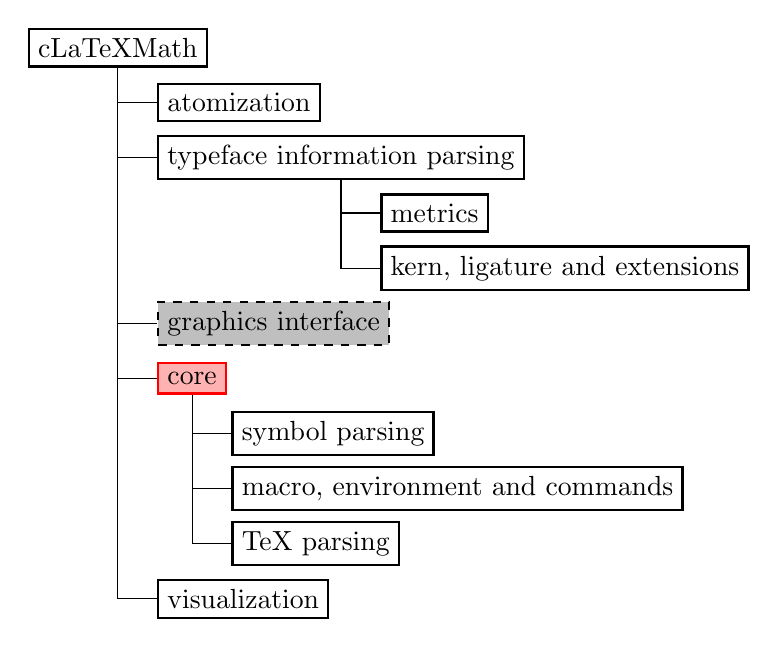
\begin{tikzpicture}[%
  grow via three points={one child at (0.5,-0.7) and
  two children at (0.5,-0.7) and (0.5,-1.4)},
  edge from parent path={(\tikzparentnode.south) |- (\tikzchildnode.west)}]
  \node {cLaTeXMath}
    child { node {atomization}}
    child { node {typeface information parsing}
        child { node {metrics}}
        child { node {kern, ligature and extensions}}
    }
    child [missing] {}
    child [missing] {}
    child { node [optional] {graphics interface}}
    child { node [selected] {core}
        child { node {symbol parsing}}
        child { node {macro, environment and commands}}
        child { node {TeX parsing}}
    }
    child [missing] {}				
    child [missing] {}				
    child [missing] {}
    child { node {visualization}};
\end{tikzpicture}
\end{center}
\end{frame}

\begin{frame}
\frametitle{\sc{extensions}}
\begin{itemize}
    \item Linux\\
    \item Windows\\
    \item Android\\
    \item Rich text\\
    \item ...
\end{itemize}
\end{frame}

%-------------------------------------------------------------------------------------------------------%


%---------------------------------------------------------------------------%

%---------------------------------------------------------------------------%


\begin{frame}{References}
\begin{thebibliography}{99}
    \bibitem{one}
        \url{http://www.sharelatex.com}
    \bibitem{two}
        \url{http://www.latex-project.org}
    \bibitem{three}
        \url{http://www.texample.net}
    \bibitem{four}
        \url{https://github.com/NanoMichael/cLaTeXMath}
\end{thebibliography}
\end{frame}
%---------------------------------------------------------------------------%

\begin{frame}
\Large
\begin{center}
 \sc { Thank You \ldots} 
\end{center}
\end{frame}
%---------------------------------------------------------------------------%
\end{CJK*}
\end{document}


